\chapter{Methodology}
\label{ch_methodology}

%This is what I did to test and confirm my hypothesis.


%You may want to split this chapter into sub chapters depending on your design. I suggest you change
%the title to something more specific to your project.

%This is where you describe your design process in detail, from component/device selection to actual
%design implementation, to how you tested your system. Remember detail is important in technical
%writing. Do not just write I used a computer give the computer specifications or the oscilloscopes part
%number. Describe the system in enough detail so that someone else can replicate your design as well
%as your testing methodology.

%If you use or design code for your system, represent it as flow diagrams in text.

\section{Outline}

This study set out to investigate the performance of modules created for a uni-directional data link in the context of laser tag systems. The following chapter presents the methodology that was followed throughout the investigation. A phased approach was taken and the following chapter gives a break down of those phases.

\begin{figure}[H]
	\centering
	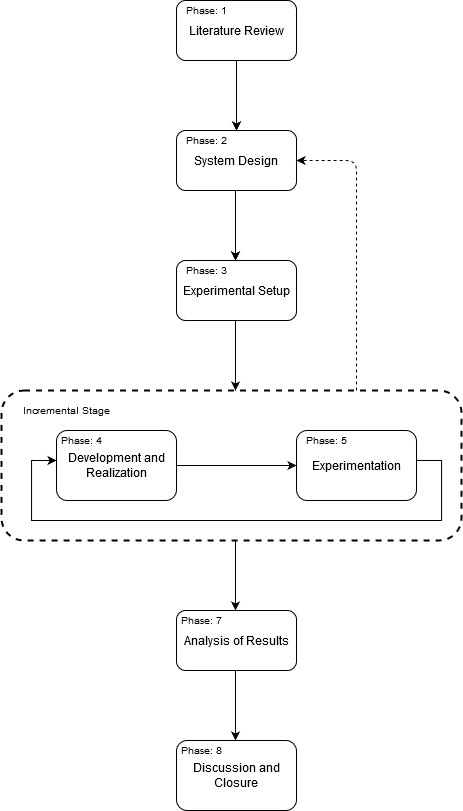
\includegraphics[width=0.5\textwidth]{figures/methodology/methodology}
	\caption{Methodology Flow Diagram}
	\label{fig:methodology_overview}
\end{figure}


The first phase involves investigating the relevant literature. The second phase involves identifying and designing the modular subsystems, this phase of the project incorporates a portion of feedback from the incremental stage. The third phase is the experimental setup during which experiments are devised and test/measurement equipment selected. Following the experimental setup is an iterative stage which comprises phase four and five. During phase four the modules are developed according to the designs produced in the second phase. Phase five then involves performing the experiments devised in the third phase to evaluate the modules.

The experimentation phase loops back to the development stage illustrating that some experiments were performed progressively as modules are realized. Following the design paradigm of the spiral model, a feedback path from the incremental stage back to the design exists to illustrated that certain design choices were made based on the experimental results.

During phase 7 the results are compiled and analysed. During the 8\textsuperscript{th} phase these results are interpreted and conclusions are drawn bringing closure to the research project.


%todo: the following sections are very 'outdated'/incomplete
\section{Phase 1 - Literature}

Lit review

Questions:

\begin{itemize}
	\item What methods exist for detection of light?
	\item ?
\end{itemize}


%%%%%%%%%%%%%%%%%%%%

\section{Phase 2 - Design}

The project can be divided into two subsystems. The tagger (transmitter) and the target (receiver). These subsystems can be further subdivided into their respective software and hardware modules. Chapter \ref{ch_design} is dedicated to this phase of the project and goes into detail on the design of these components.

\begin{figure}[H]
	\centering
	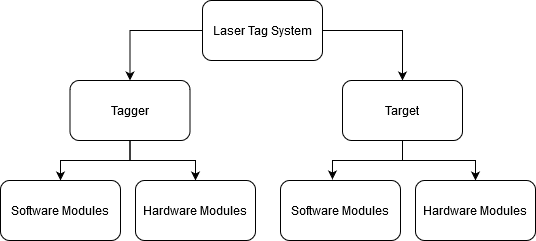
\includegraphics[width=0.7\linewidth]{figures/methodology/design_overview}
	\caption{Design Overview}
	\label{fig:designoverview}
\end{figure}

Figure \ref{fig:designoverview} provides a breakdown of the systems high-level design requirements.


%%%%%%%%%%%%%%%%%%%%

\section{Phase 3 - Experimental Setup}

The investigation required various pieces of test and measurement equipment. The following section outlines the hardware and software used to develope the system and perform the experiments.

\subsection{Power Supply}
Access to the university laboratory equipment is limited.

A large potion of the testing will be done using a custom built power supply, created from an ATX PSU. The particular unit that was repurposed was a 280W LiteOn PSU. This unit is capable of supplying $\pm$ 12V, $\pm$ 5V, and 3.3V.

On occasion when a variable power supply was required, XXX

\subsection{Measurement}

Various experiments required the use of an oscilloscope, the oscilloscope used was the PicoScope 2205A by Pico Technology.

For general purpose measurements of voltages, current and resistance the Fragram T2612 digital multimeter was used.

A large portion of the project is centred around invisible IR radiation. To measure the characteristics such as the beam angle produced by the IR, the Sony Handycam DCR-HC26 was used. To maximize the visibility of the IR beam, the camera was operated in 'Nightshot' mode and the built in IR LEDs covered up.



%%%%%%%%%%%%%%%%%%%%

\subsection{Hardware Components}

\subsubsection{UCT STM32F0 Development Board}
The STM32F051C6 microcontroller was chosen due to its combination of low cost and availability. UCT has a custom design development board centred on this microcontroller. The final prototype is centred purely on the STM32F0 microcontroller and bare-bones supporting circuity, however a vast amount of the testing was done on the development board hence its inclusion in this section.

%\subsubsection{ADC Peripheral}

%\subsubsection{ADC DMA}

%\subsection{Arduino}
%The Arduino platform was used whenever for various quick prototyping where unofficial testing was required. This is because the Arduino platform has many well established libraries and a simplified development environment which allowed for faster prototyping.

\subsubsection{Power IR LED}

The LZ1-10R702 high power, PCB mounted LED from LedEngin Inc. was used to produce the required 940nm wavelength infrared radiation. To ensure proper heat dissipation generic adhesive based heat-sink was attached to the module.

\subsubsection{Operational Amplifier}
xxx

\subsubsection{LED Current Regulator}
xxx
IRLZ44NPBF N-Channel MOSFET from Infineon



%%%%%%%%%%%%%%%%%%%%

\subsection{Software Applications}

\subsubsection{STM32 CubeIDE}
ST microelectronics provides a custom version of the Eclipse IDE, distributed under the name CubeIDE. This is an all in one integrated developer environment for STM32 microcontrollers. Version 1.3.0 was used for the software development in this study.

CubeIDE provides a 'Device Configuration Tool' along with an official library called HAL (Hardware Abstraction Layer). The combination of the configuration tool and HAL library helped speed up the software development. The CubeIDE also includes a debug tool with direct register/memory access which assisted with debugging.

XXX -talk about LCD libary

\subsubsection{Realterm}
During the development and realization stage a UART communication link between the personal computer and the micro-controller was used to provide feedback and measurements. Realterm \footnote{\url{https://sourceforge.net/projects/realterm/}}, a free serial monitor which provides a rich set of features was used for these communications.

\subsubsection{Git}



%%%%%%%%%%%%%%%%%%%%

\section{Phase 4 - Development and Realization}

The development and realization phase forms part of the iteration stage. The laser tag system will be developed in a progressive fashion. After each module is realized, a set of experiments will be undertaken to assess the module's performance. This phase involves the creation of both hardware and software modules.

\section{Phase 5 - Experimentation}
%Experimentation will achieve two goals, validation/verification and performance testing.

The experimentation phase will aim to gather data to be used to answer the 



\section{Phase 7 - Analysis of Results}



\section{Phase 8 - Discussion and Closure}








